%%%%%%%%%%%%%%%%%%%%%%%%%%%%%%%%%%%%%%%%%
% Short Sectioned Assignment
% LaTeX Template
% Version 1.0 (5/5/12)
%
% This template has been downloaded from:
% http://www.LaTeXTemplates.com
%
% Original author:
% Frits Wenneker (http://www.howtotex.com)
%
% License:
% CC BY-NC-SA 3.0 (http://creativecommons.org/licenses/by-nc-sa/3.0/)
%
%%%%%%%%%%%%%%%%%%%%%%%%%%%%%%%%%%%%%%%%%

%----------------------------------------------------------------------------------------
%	PACKAGES AND OTHER DOCUMENT CONFIGURATIONS
%----------------------------------------------------------------------------------------

\documentclass[paper=a4, fontsize=10pt]{scrartcl} % A4 paper and 11pt font size


\usepackage[T1]{fontenc} % Use 8-bit encoding that has 256 glyphs
\usepackage[english,francais]{babel} % Français et anglais
\usepackage[utf8]{inputenc} 

\usepackage{amsmath,amsfonts,amsthm} % Math packages

\usepackage{lmodern}
\usepackage{url}
\usepackage{eurosym} % signe Euros
\usepackage{geometry} % Pour passer au format A4
\geometry{a4paper} % 
\usepackage{graphicx} % Required for including pictures
\usepackage{float} % Allows putting an [H] in \begin{figure} to specify the exact location of the figure

\usepackage{multicol}
\usepackage{sectsty} % Allows customizing section commands
\allsectionsfont{\centering \normalfont\scshape} % Make all sections centered, the default font and small caps

%----------------------------------------------------------------------------------------
%	Pied de Page
%----------------------------------------------------------------------------------------


\usepackage{fancyhdr} % Custom headers and footers
\pagestyle{fancyplain} % Makes all pages in the document conform to the custom headers and footers
\fancyhead{} % No page header - if you want one, create it in the same way as the footers below
\fancyfoot[L]{$5^{e}1$} % Empty left footer
\fancyfoot[C]{Chapitre 9 - Angles et parallélisme} % Empty center footer
\fancyfoot[R]{\thepage} % Page numbering for right footer

\renewcommand{\headrulewidth}{0pt} % Remove header underlines
\renewcommand{\footrulewidth}{0pt} % Remove footer underlines

\setlength{\headheight}{13.6pt} % Customize the height of the header


\setlength\parindent{0pt} % Removes all indentation from paragraphs - comment this line for an assignment with lots of text


%----------------------------------------------------------------------------------------
%	Titre
%----------------------------------------------------------------------------------------

\newcommand{\horrule}[1]{\rule{\linewidth}{#1}} % Create horizontal rule command with 1 argument of height


\title{	
  \vspace{-10ex}
  \horrule{0.5pt} \\[0.4cm] % Thin top horizontal rule
  \huge Chapitre 9 - Angles et parallélisme\\ % The assignment title
  \horrule{2pt} \\[0.5cm] % Thick bottom horizontal rule
}

\author{}
\date{\vspace{-10ex}} % Today's date or a custom date

%----------------------------------------------------------------------------------------
%	Début du document
%----------------------------------------------------------------------------------------

\begin{document}

%----------------------------------------------------------------------------------------
% RE-DEFINITION
%----------------------------------------------------------------------------------------
% MATHS
%-----------

\newtheorem{Definition}{Définition}
\newtheorem{Theorem}{Théorème}
\newtheorem{Proposition}{Propriété}

% MATHS
%-----------
\renewcommand{\labelitemi}{$\bullet$}
\renewcommand{\labelitemii}{$\circ$}
%----------------------------------------------------------------------------------------
%	Titre
%----------------------------------------------------------------------------------------

\maketitle % Print the title



%-----------------------------------111111111111111111111111111111111111
\section{Angles}
%----------------------------------------------------------------------

\subsection{Angles adjacents}
\begin{multicols}{2}

  \begin{Definition}{Angles adjacents}\\
    Deux angles sont adjacents si :
    \begin{itemize}
    \item Ils ont un même sommet;
    \item Ils ont un côté commun;
    \item Ils sont situés de part et d'autre de ce côté commun.
    \end{itemize}
  \end{Definition}

  \begin{figure}[H]
    \centering
    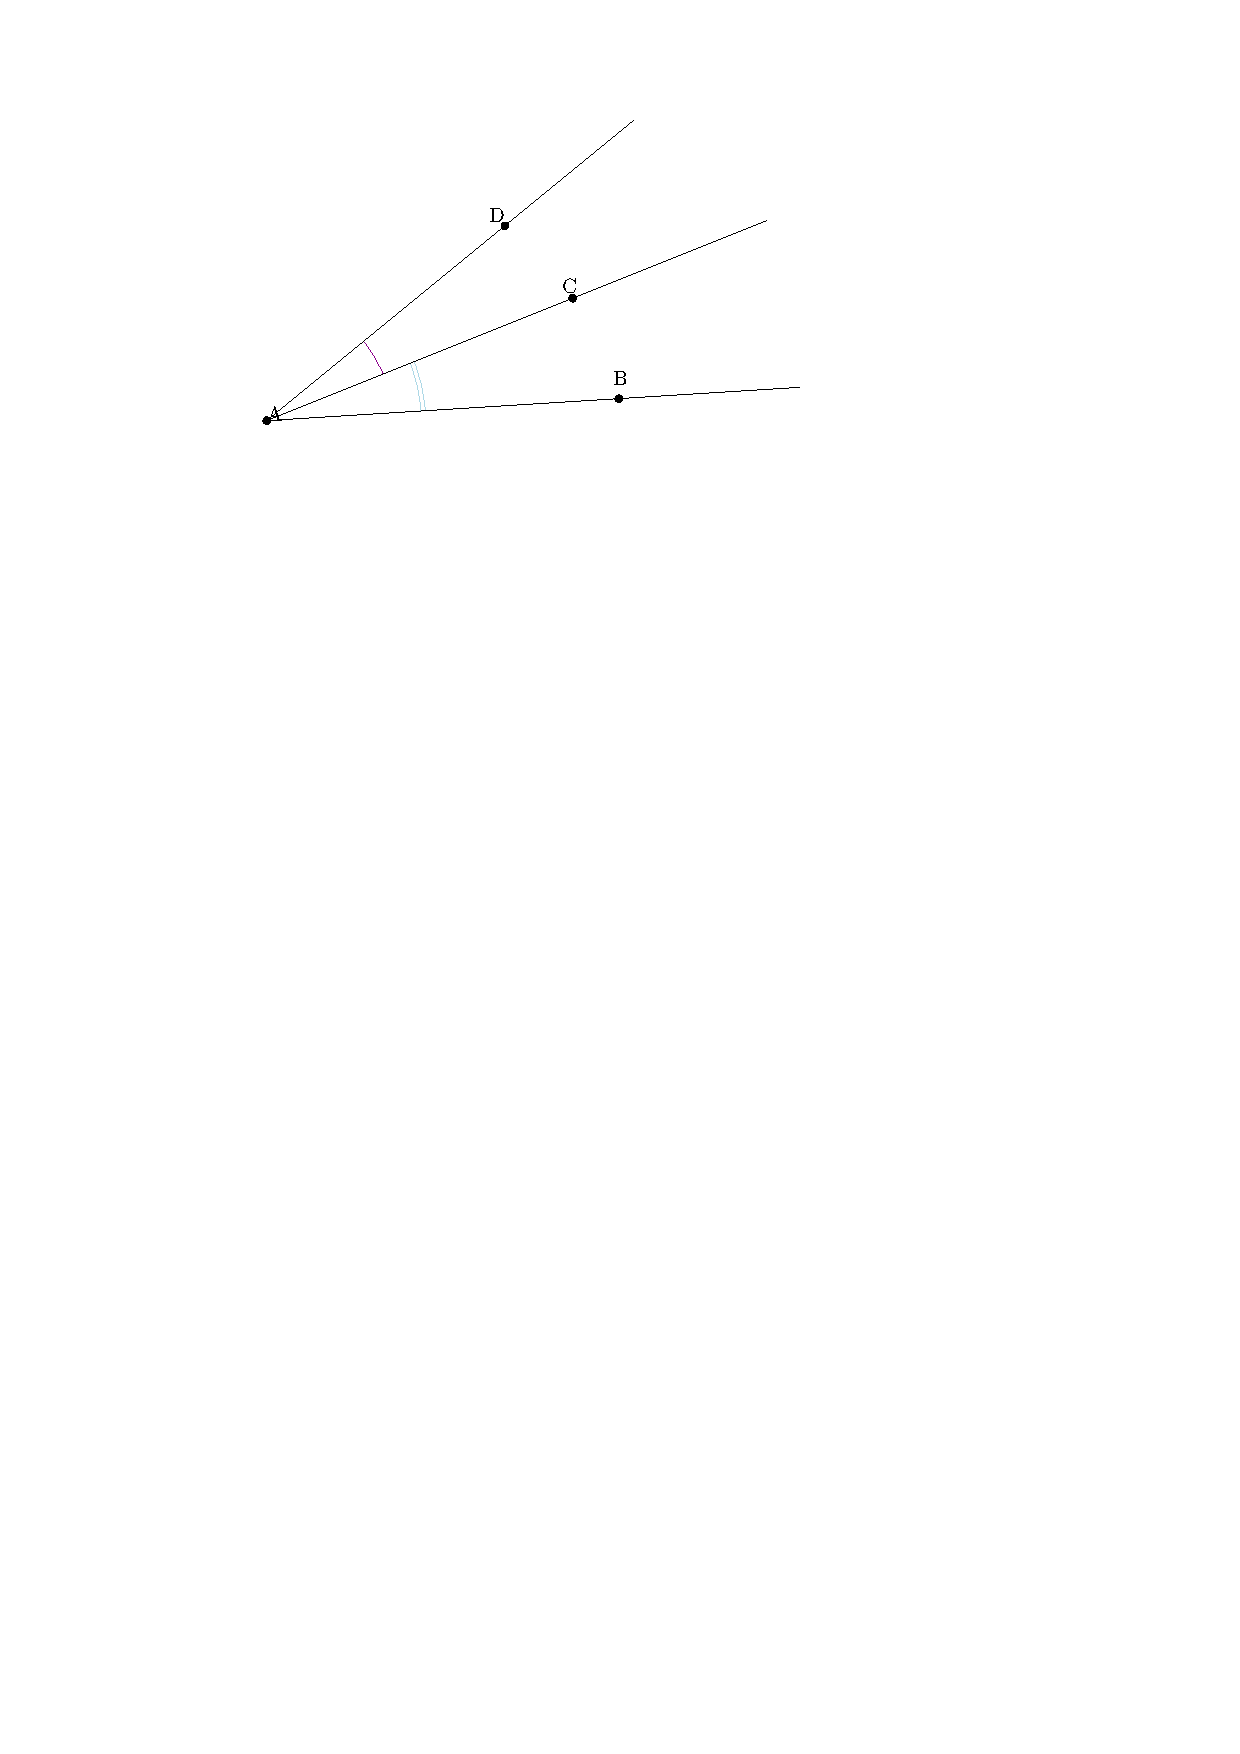
\includegraphics[width=0.8\linewidth]{sources/cours/adjacents.pdf}
  \end{figure}
\end{multicols}

\subsection{Angles opposés par le sommet}
\begin{multicols}{2}
  \begin{Definition}{Angles opposés par le sommet}\\
    Deux angles sont opposés par le sommet si :
    \begin{itemize}
    \item Ils ont un même sommet;
    \item Les côtés de l'un sont le prolongement des côtés de l'autre.
    \end{itemize}
  \end{Definition}
  \begin{figure}[H]
    \centering
    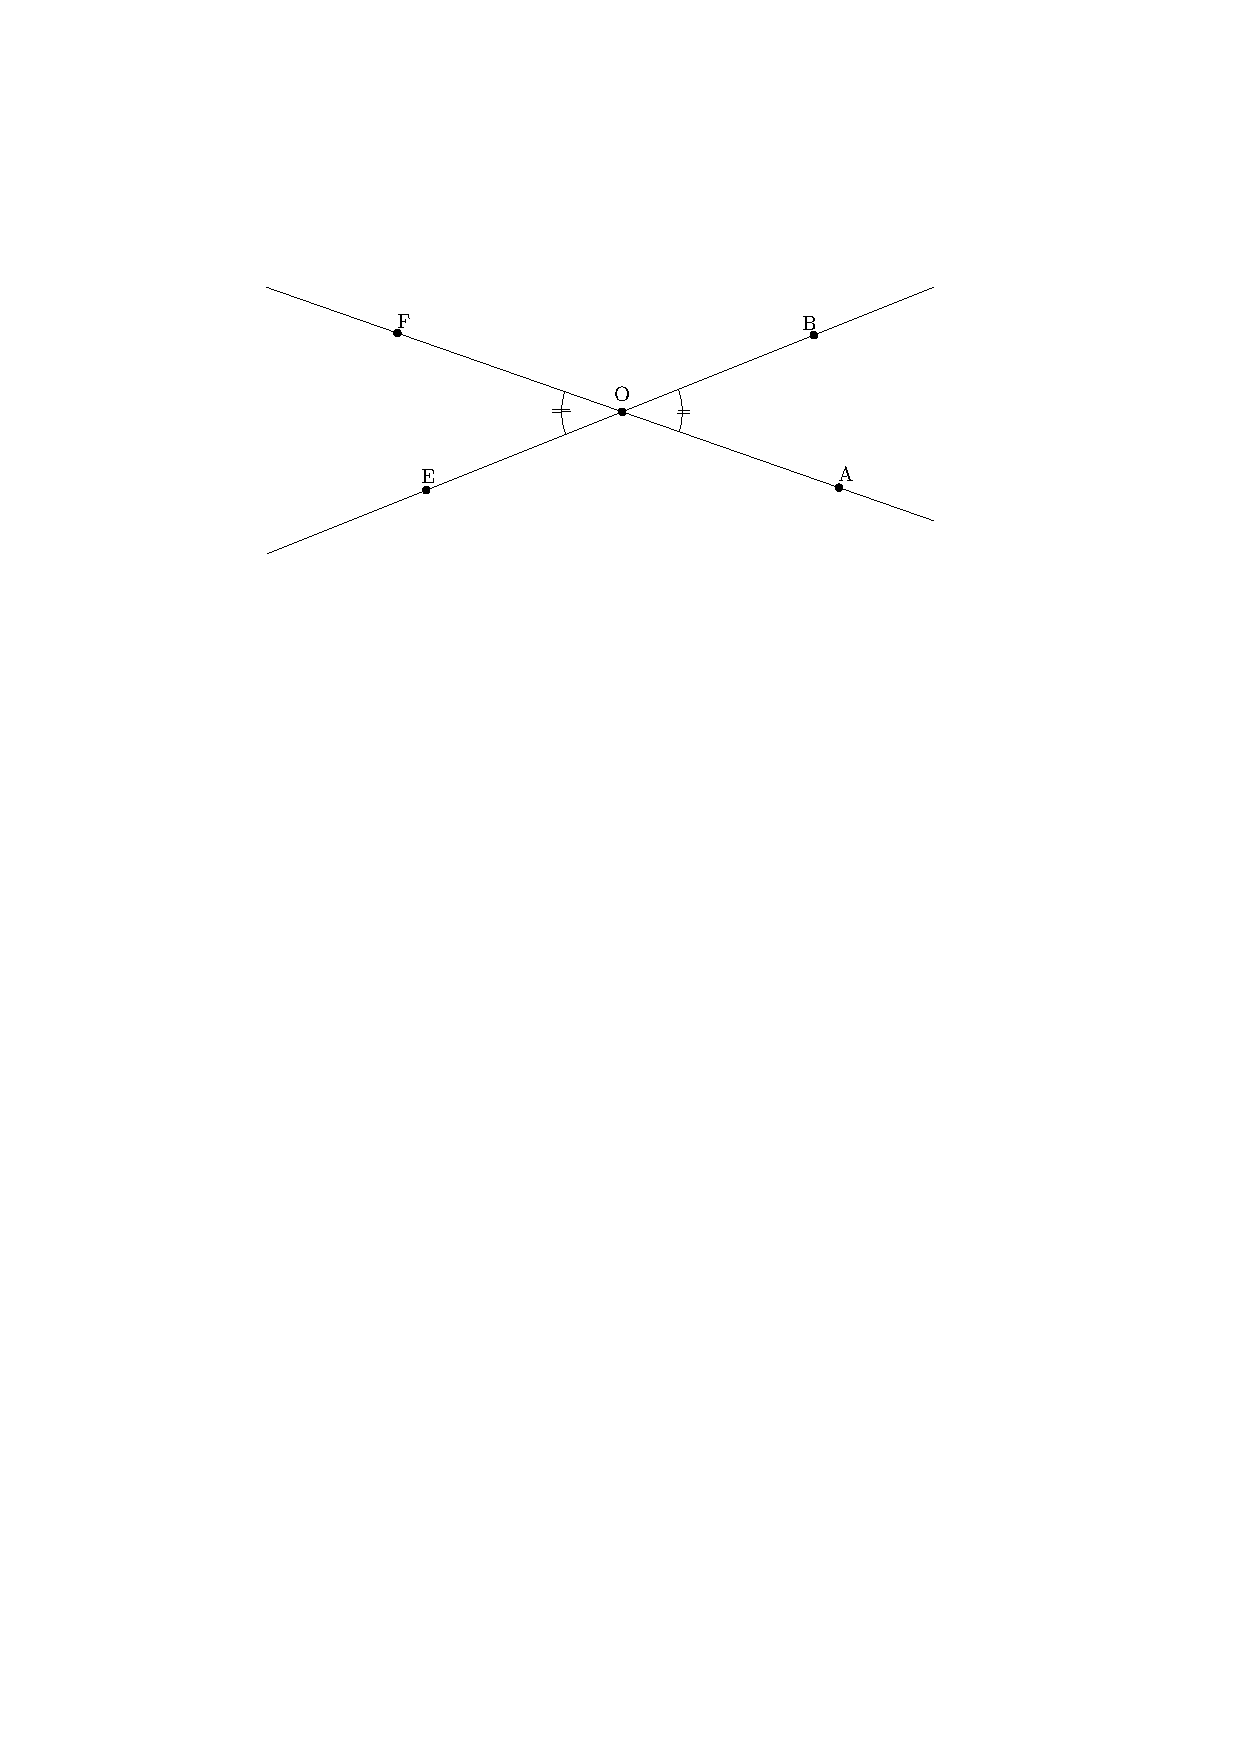
\includegraphics[width=0.8\linewidth]{sources/cours/opposes.pdf}
  \end{figure}
\end{multicols}

\begin{Proposition}
  Deux angles opposés par le sommet sont égaux.
\end{Proposition}


\subsection{Angles complémentaires}
\begin{multicols}{2}

  \begin{Definition}{Angles complémentaires}\\
    Deux angles sont complémentaires si la somme de leurs mesures est égale à 90\char6.
  \end{Definition}
  \begin{figure}[H]
    \centering
    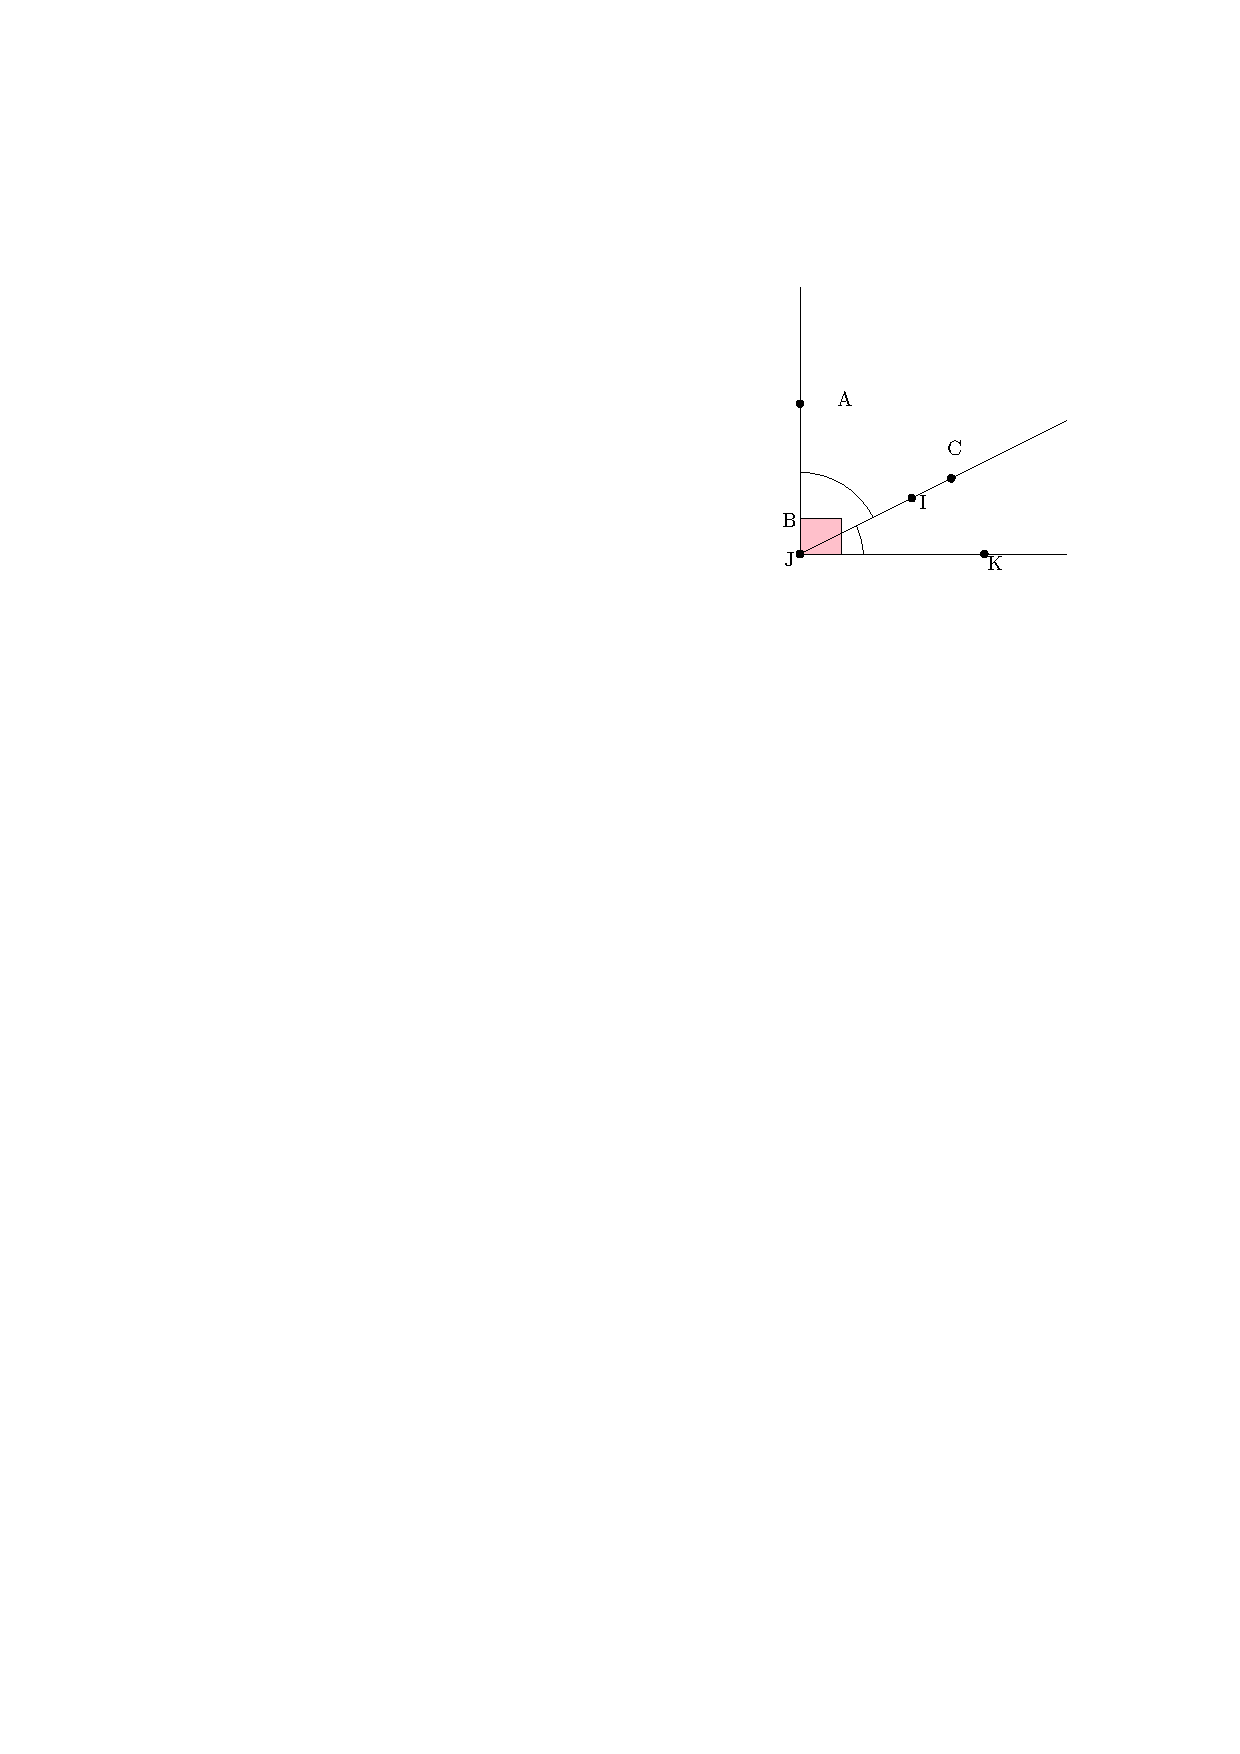
\includegraphics[width=0.6\linewidth]{sources/cours/complementaires.pdf}
  \end{figure}
\end{multicols}

\subsection{Angles supplémenaitres}
\begin{multicols}{2}
  \begin{Definition}{Angles supplémentaires}\\
    Deux angles sont supplémentaires si la somme de leurs mesures est égale à 180\char6.
  \end{Definition}
  \begin{figure}[H]
    \centering
    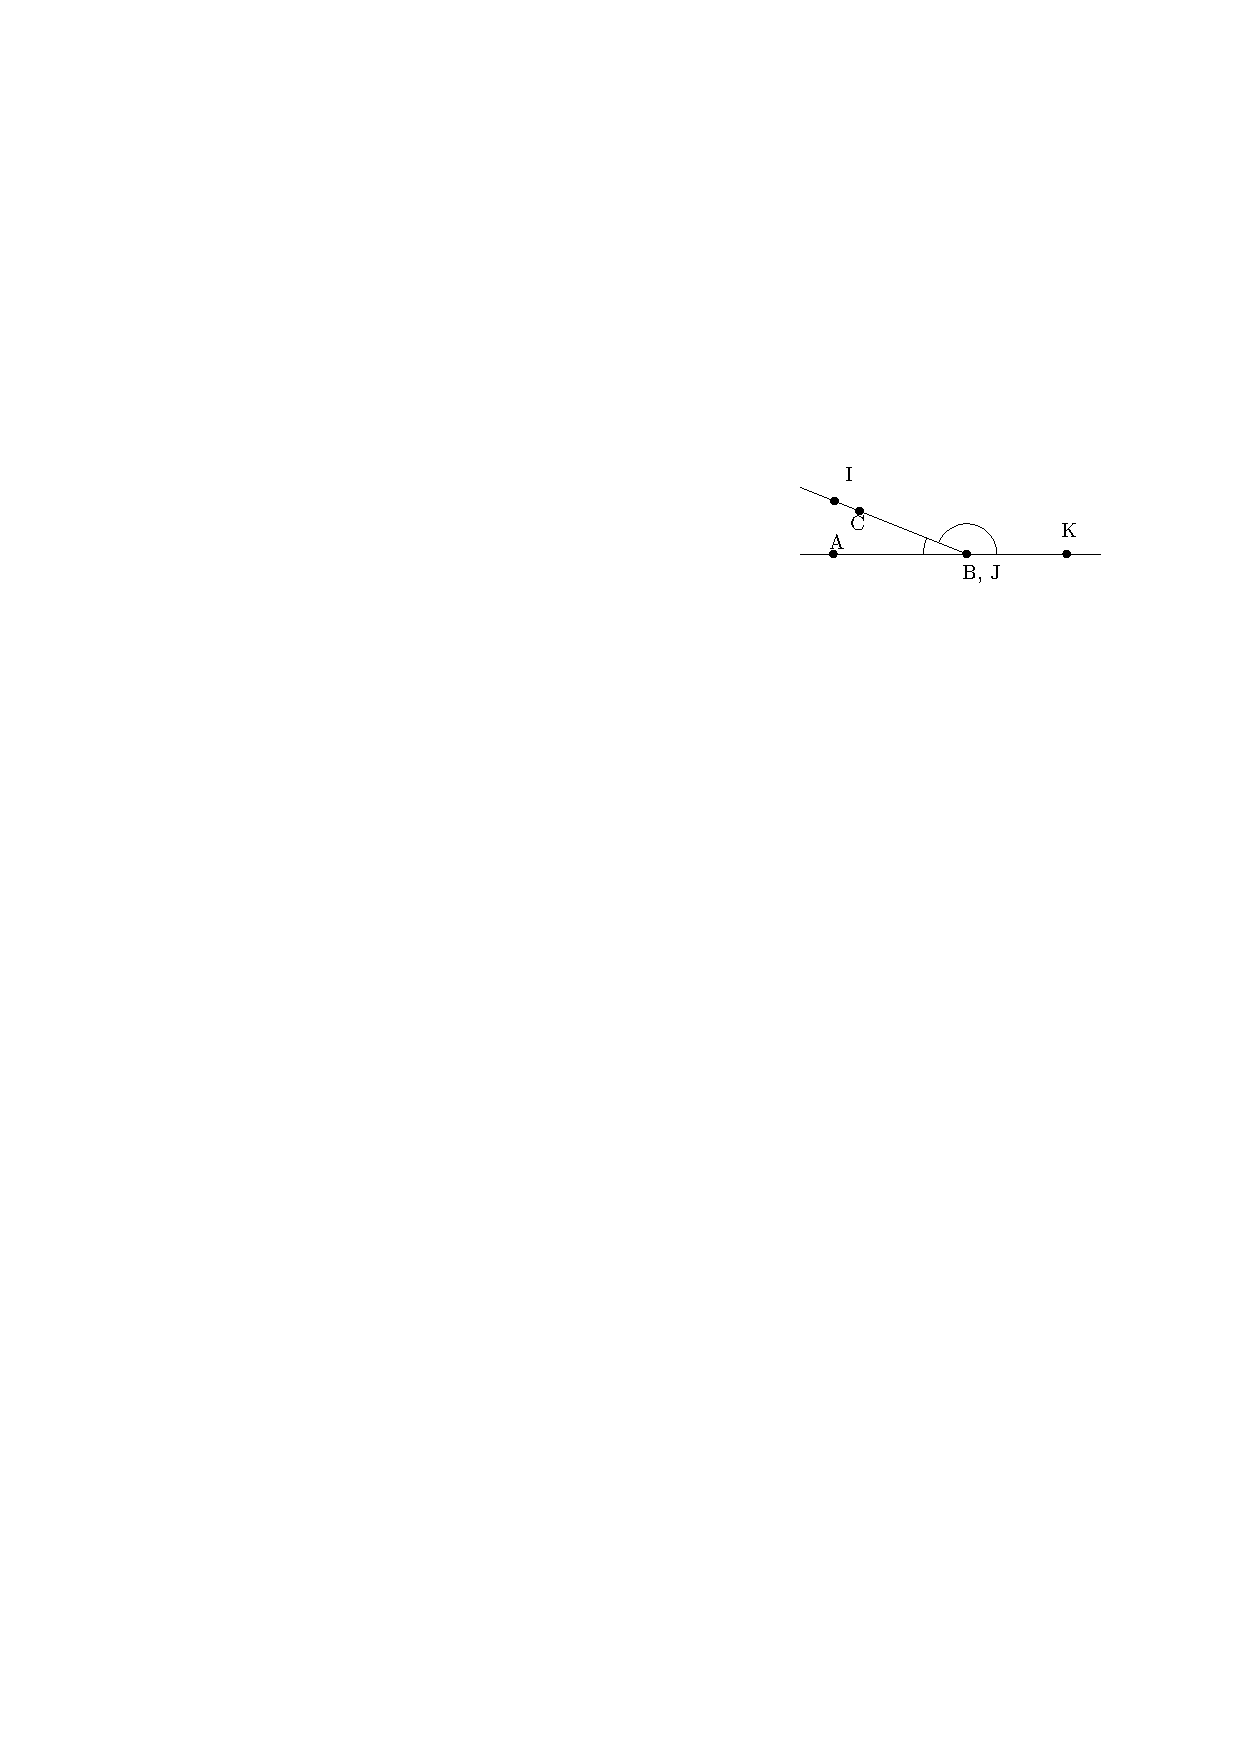
\includegraphics[width=0.8\linewidth]{sources/cours/supplementaires.pdf}
  \end{figure}
\end{multicols}


%-----------------------------------111111111111111111111111111111111111
\section{Angles et parallélisme}
%----------------------------------------------------------------------

Soient deux droites $d_1$ et $d_2$ coupées par une troisième droite $d_3$.
\subsection{Angles alternes-internes}
\begin{multicols}{2}
  \begin{figure}[H]
    \centering
    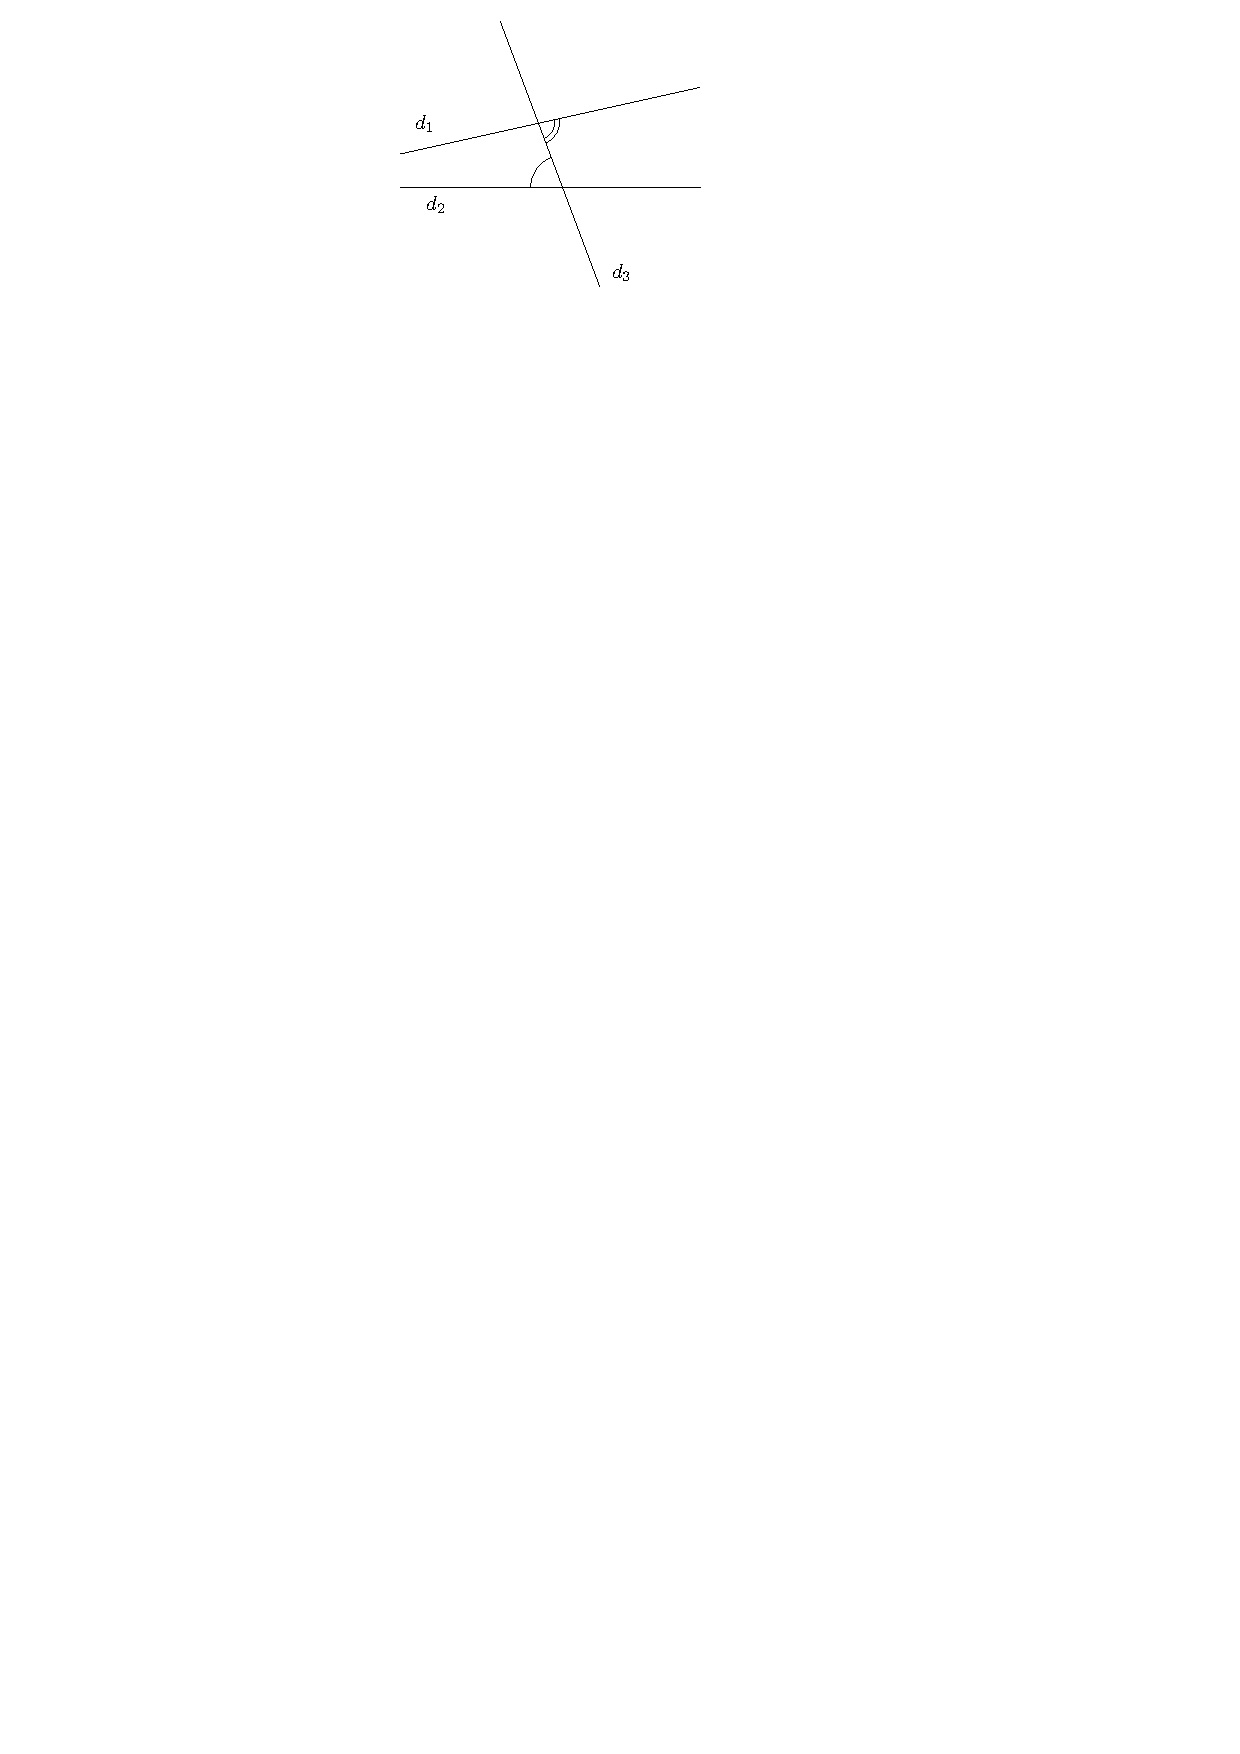
\includegraphics[width=0.8\linewidth]{sources/cours/ai-1.pdf}
  \end{figure}
  \begin{figure}[H]
    \centering
    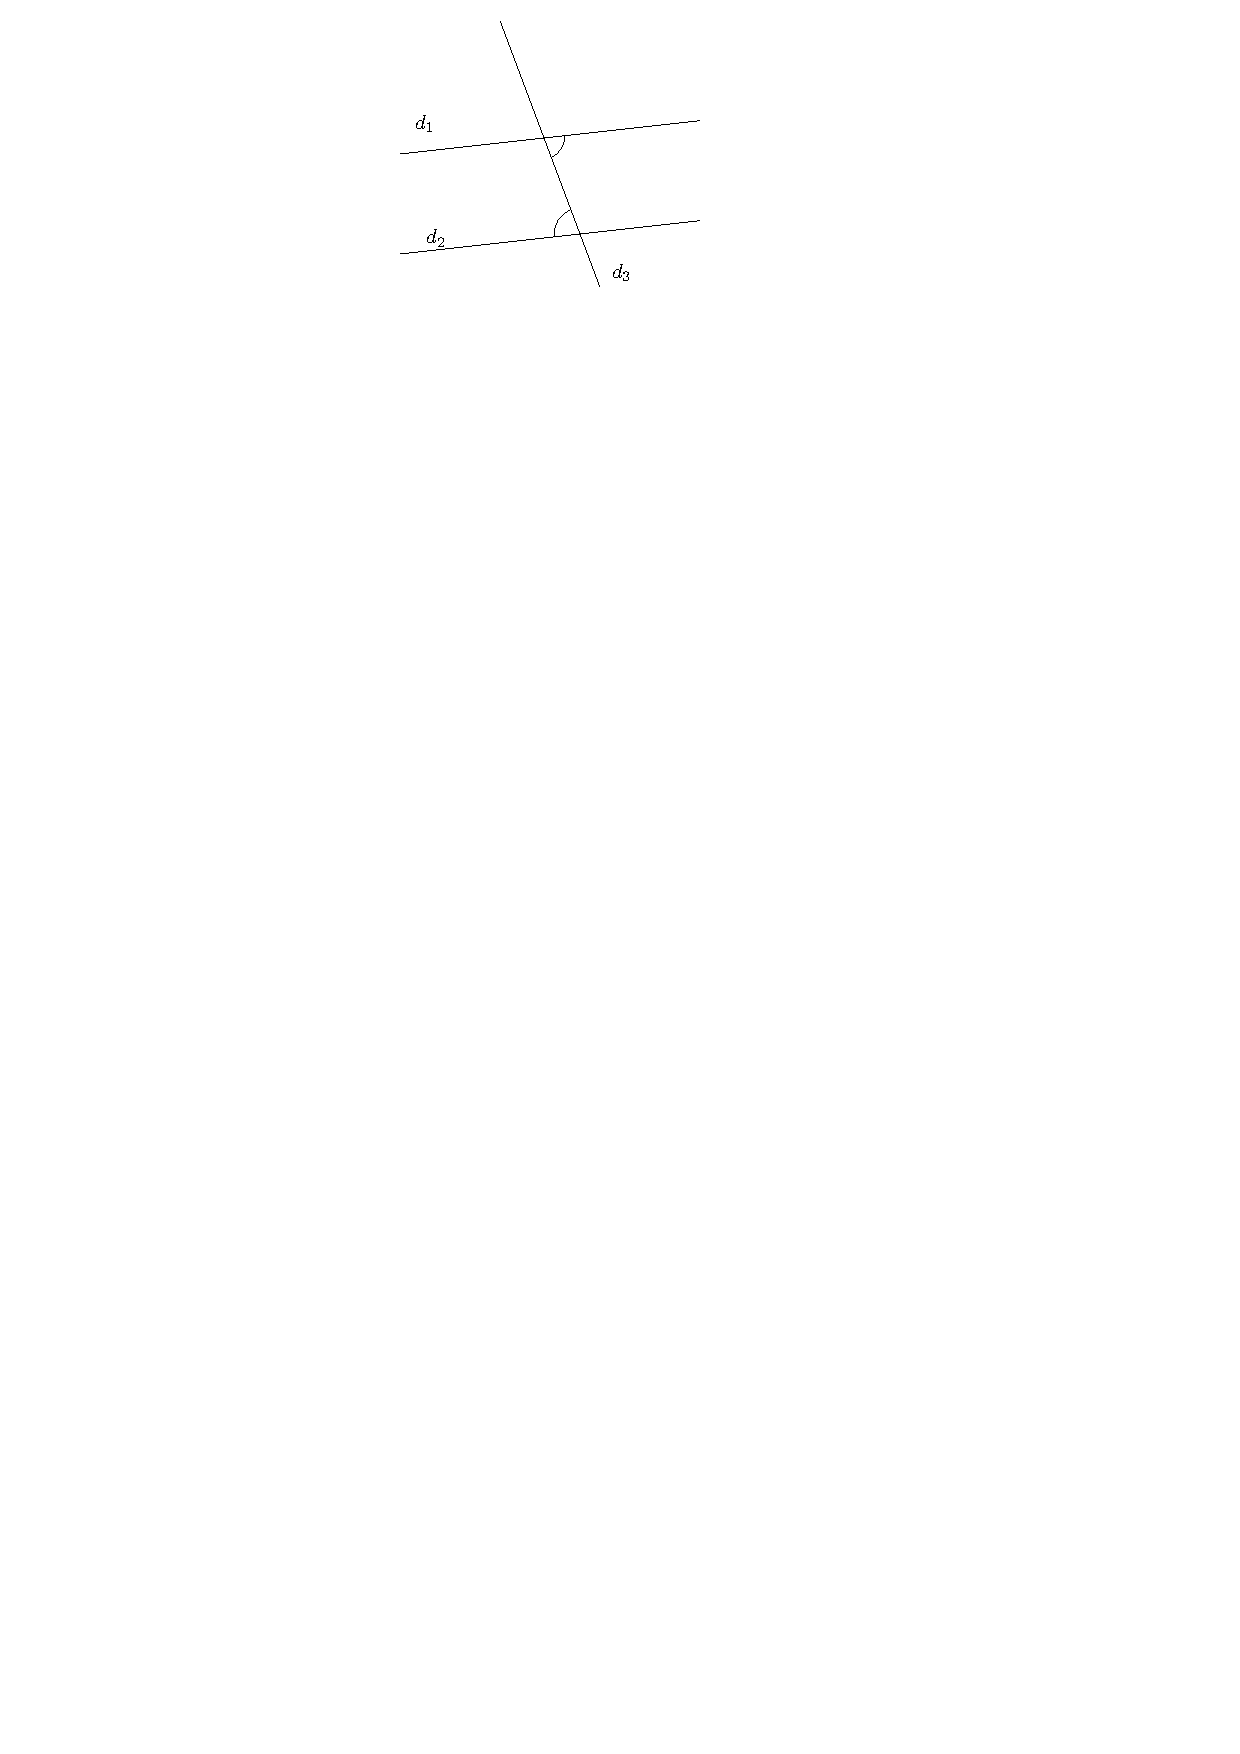
\includegraphics[width=0.8\linewidth]{sources/cours/ai-2.pdf}
  \end{figure}
\end{multicols}
\begin{multicols}{2}
  \begin{Definition}{Angles alternes-internes}\\
  \end{Definition}

  \begin{Proposition}{$d_1$ et $d_2$ sont parallèles.}\\
    Les angles alternes-internes sont égaux.
  \end{Proposition}
\end{multicols}
\subsection{Angles correspondants}
\begin{multicols}{2}
  \begin{figure}[H]
    \centering
    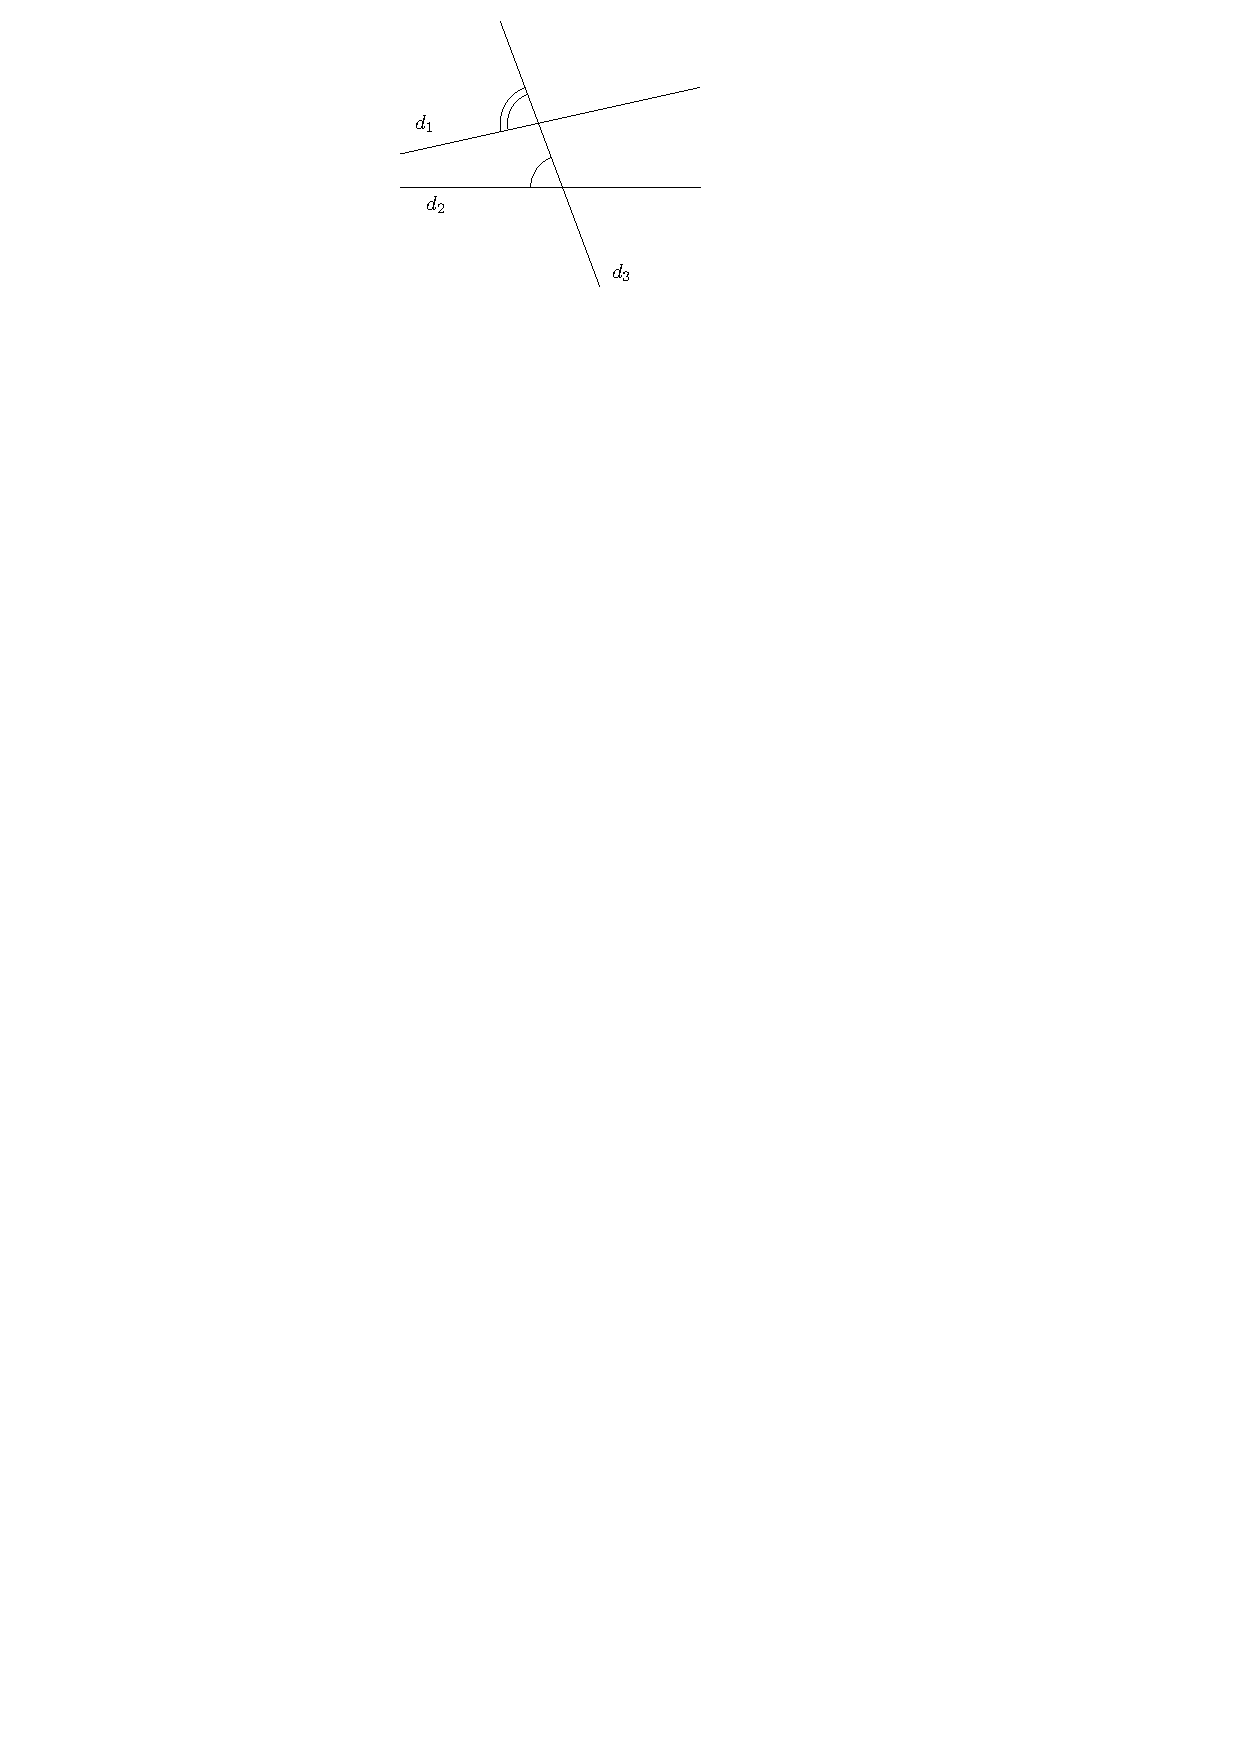
\includegraphics[width=0.8\linewidth]{sources/cours/corres-1.pdf}
  \end{figure}
  \begin{figure}[H]
    \centering
    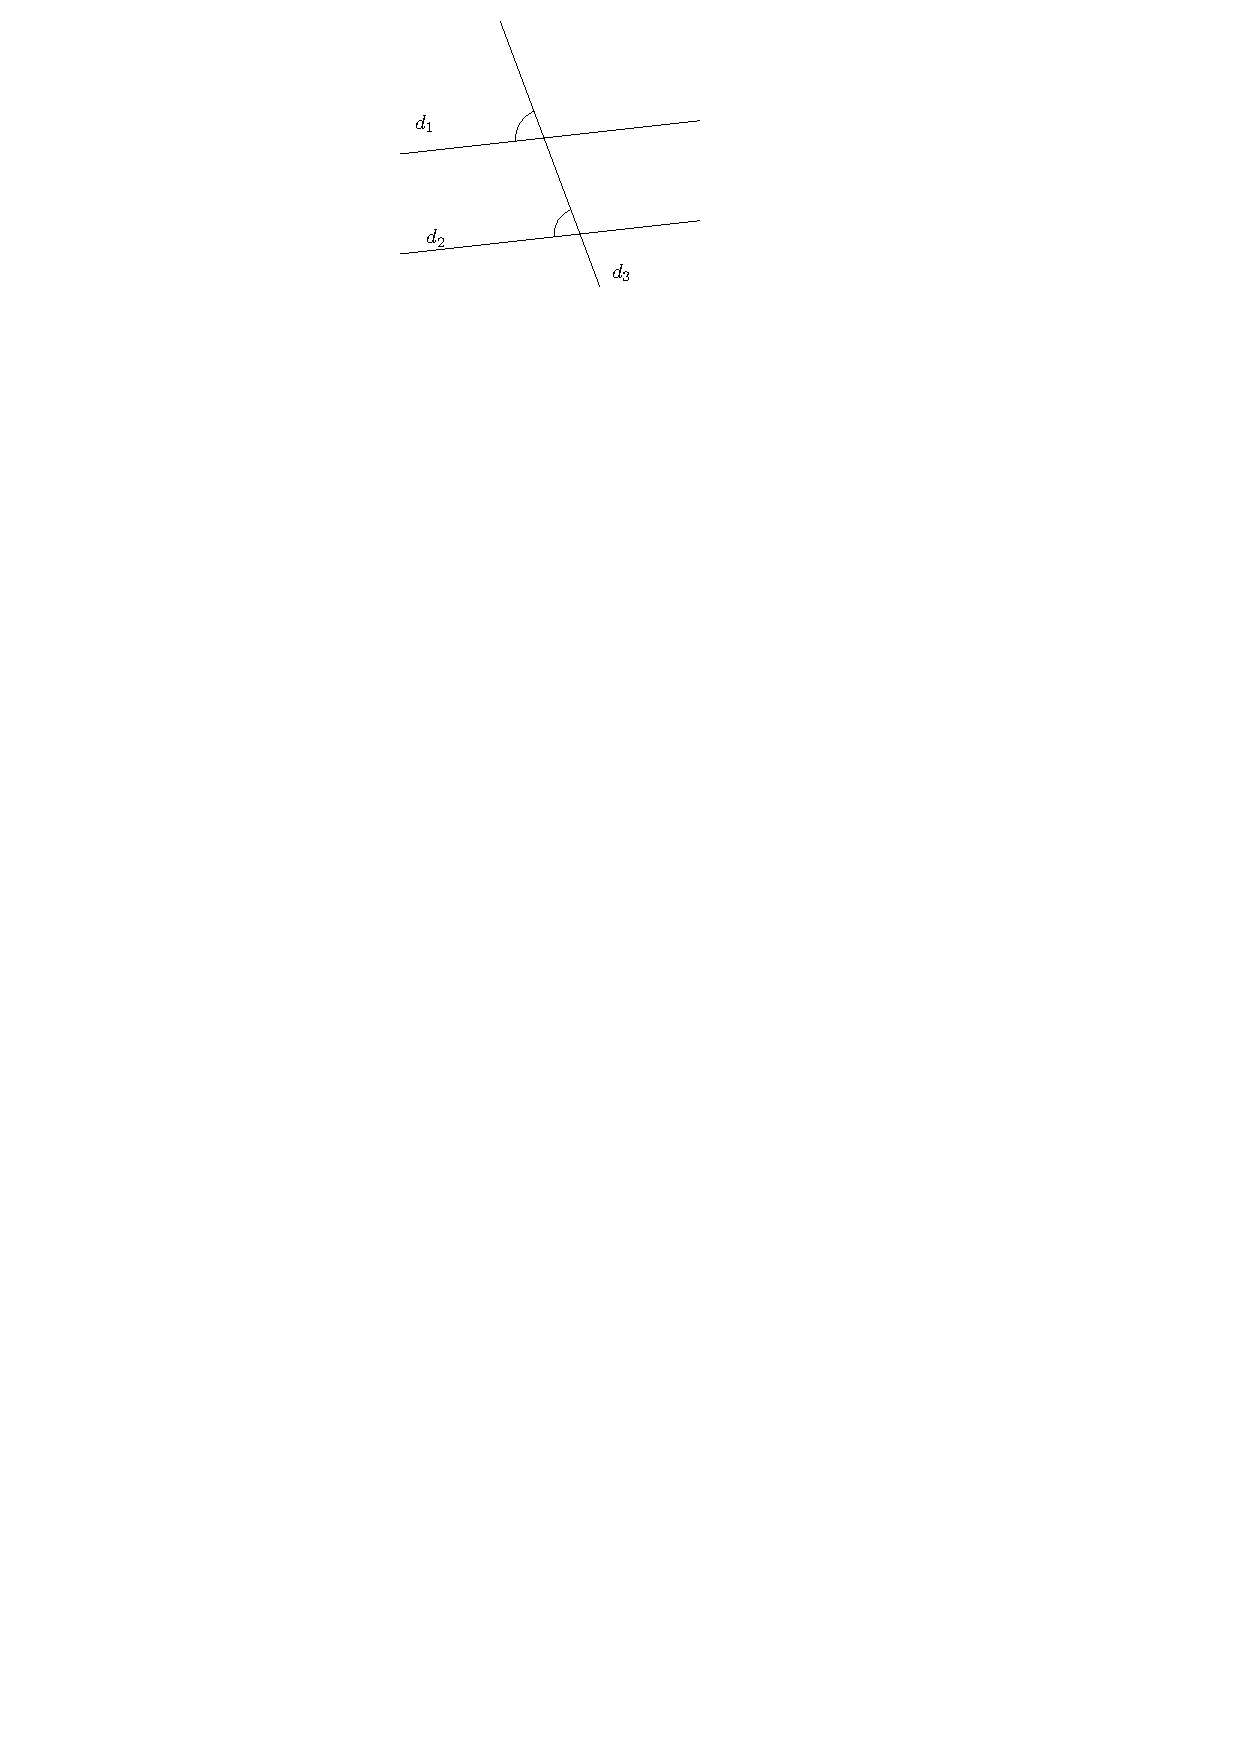
\includegraphics[width=0.8\linewidth]{sources/cours/corres-2.pdf}
  \end{figure}
\end{multicols}

\begin{multicols}{2}
  \begin{Definition}{Angles correspondants}\\
  \end{Definition}

  \begin{Proposition}{$d_1$ et $d_2$ sont parallèles.}\\
    Les angles correspondants sont égaux;
  \end{Proposition}
\end{multicols}



\end{document}
